\chapter{Energía eléctrica y desarrollo sostenible.}
\section{Introducción al desarrollo sostenible.}
El desarrollo nació en los años 70 en los países nórdicos y se define como:
\begin{itemize}
	\item [-] El que satisface
	nuestras necesidades actuales sin poner en peligro la
	capacidad de las generaciones futuras para satisfacer sus
	propias necesidades abarcando:
	\begin{itemize}
		\item El capital social
		\item El capital ambiental
		\item El capital económico
	\end{itemize}
\end{itemize}
\subsection{Cumbres climáticas.}
\begin{itemize}
	\item [-] \textbf{Rio de Janeiro (1992):}
		Se crea la Comisión del Desarrollo Sostenible para impulsar la sostenibilidad de las políticas de desarrollo humano y gestionar sus riesgos.
	\item [-] \textbf{Cumbre del Protocolo de Kyoto (1997):}
		Se adquiere un compromiso entre los países industrializados con el \textbf{objetivo} de reducir las emisiones de gases de efecto invernadero un 5,9\% en el periodo 2008 - 2012 con respecto a 1990 (año base). En una fase inicial no incluía a países en desarrollo como China e India por su baja contaminación per capita.
	\item [-] \textbf{Cumbre de París (2015):}
		Se comprometen los países a que la temperatura mundial no aumente más de 2\textdegree C respecto a los niveles preindustriales y limitarlo a 1,5\textdegree C para el 2020.
	\item [-] \textbf{Cumbre de Marrakech (2016):}
		Se ratifican los acuerdos de la Cumbre de París y se compromete reducir el 80\% de las emisiones de CO$_2$ para 2050.
	\item [-] \textbf{Cumbre de Katowice (2018):}
		Limitar a un incremento a final de siglo de 1,5 a 2\textdegree C respecto a los niveles preindustriales.
	\item [-] \textbf{Cumbre de Chile celebrada en Madrid (2019):}
		Los grandes contaminadores se niegan a intensificar los esfuerzos para mantener la temperatura por debajo de 1,5\textdegree C.
	\item [-] \textbf{Cumbre de Glasgow (2021):}
		Se mantiene el objetivo de 1,5\textdegree C para 2030. Acuerdo China - USA para reducir las emisiones de metano. Compromiso de 130 países para poner fin a la deforestación.
	\item [-] \textbf{Cumbre de Sharm el-Sheij en Egipto (2022):}
		Se acuerdan:
		\begin{itemize}
			\item Una alianza global contra la sequía.
			\item Una coalición contra la deforestación.
			\item Impulsar el hidrógeno verde.
			\item Impulsar la energía eólica marina.
		\end{itemize}
	\item [-] \textbf{Cumbre de Dubai(2021):}
		Se acuerda reducir las emisiones mundiales de gases de efecto invernadero un 43\% hasta
		2030 y un 60\% hasta 2035 en relación con los niveles de 2019, y emisiones netas de dióxido de carbono cero
		para 2050.
\end{itemize}
\section{Gases de efecto invernadero.}
\subsection{CO$_2$ equivalente.}
Es una forma de poder reducir el impacto climático a una unidad común y así, poder compararlos. Para calcularlo se emplea el valor \textbf{GWP} (Global Warming Potencial) o \textbf{PCG} (Potencial de calentamiento global) que miden cuanto calor atrapan en comparación con el CO$_2$ para un periodo de tiempo. 


Este valor depende de:
\begin{itemize}
	\item [-] La absorción de radiación infrarroja.
	\item [-] La ubicación del espectro de absorción.
\end{itemize}
\subsection{Dióxido de carbono (CO$_2$).}
Es la sustancia que más contribuye al efecto invernadero. Absorbe gran parte de la radiación solar incidente.
\subsection{Óxido nitroso (N$_2$O) y óxidos de nitrógeno (NO$_x$ ).}
Son los gases de efecto invernadero más destructivos con la capa de ozono. Relacionados con el sector agrario y la quema de combustible.
\subsection{Metano (CH$_4$).}
Tiene un potencial de calentamiento muy elevado GWP = 25. Se emite por el sector ganadero, el el de tratamiento de residuos y durante el transporte de hidrocarburos.
\subsection{Hidrofluorocarbonos (HFC).}
Son gases empleados como refrigerantes. No dañan al ozono pero tienen un GWP = 1000 y una larga permanencia en la atmósfera.
\subsection{Perfluororcarburos (PFC).}
Similares a los HFC.
\subsection{Hexafluoruro de azufre (SF$_6$).}
Se emplea para equipos de distribución de energía eléctrica. Tiene propiedades similares a los HFC y PFC.

\begin{table}[H]
	\centering
	\begin{tabular}{p{2cm}p{2cm}p{2cm}p{2cm}p{2cm}}
		\hline
		\textbf{ } & \textbf{CO$_2$} & \textbf{ClFCs} & \textbf{CH$_4$} & \textbf{N$_2$O} \\ \hline
		Importancia según contribución al efecto invernadero & Más del 50\% & 20 \% aprox. & 12 a 14 \% & 6 a 7 \% \\ \hline
		Tiempo de permanencia en la atmósfera & 50 - 200 años & 75 - 100 años & 7 a 10 años & 150 años aprox. \\ \hline
		Tasa de crecimiento anual (\%)&0,5&4-5&1&0,35\\ \hline 
		Principal origen de la contaminación&Combustión del petróleo, carbón y gas deforestación&Aerosoles y disolventes Espumas industriales Equipos de refrigeración&Pantanos Ganadería Minería&Fertilizantes Combustible fósiles\\ \hline 
	\end{tabular}
	\label{tab:my-table}
\end{table}

\section{Efecto invernadero.}
Como consecuencia de los gases de efecto invernadero se absorbe una mayor cantidad de radiación infrarroja que escaparía de la tierra y, por tanto, aumentando la temperatura atmosférica. 
\begin{figure}[H]
	\centering
	\includegraphics[width=0.7\linewidth]{res/tema2/T-Emisiones}
	\label{fig:t-emisiones}
\end{figure}
\subsection{Forzamiento radiactivo o climático.}
Es la diferencia entre la radiación solar absorbida por la Tierra y la energía irradiada de vuelta al espacio. Esta diferencia se contempla mediante el RCP donde:
\begin{itemize}
	\item [-] RCP = 2 es un escenario con el indicador muy bajo.
	\item [-] RCP = 8,5 es un escenario con el indicador muy alto.
\end{itemize}

\begin{table}[h]
	\centering
	\renewcommand{\arraystretch}{1.5}
	\begin{tabular}{cccccc}
		\hline
		Escenario & Forz. Radiat. (W/m\textsuperscript{2} en 2100) & \multicolumn{2}{c}{GC} & \multicolumn{2}{c}{GtCO$_2$} \\
		\cline{3-6}
		& &Media & Rango & Media & Rango \\
		\hline
		RCP2.6 & 2.8 & 270 & 140 a 410 & 990 & 510 a 1505 \\
		RCP4.5 & 4.5 & 780 & 595 a 1005 & 2880 & 2180 a 3690 \\
		RCP6.0 & 6 & 1060 & 840 a 1250 & 3885 & 3080 a 4585 \\
		RCP8.5 & 8.5 & 1685 & 1415 a 1910 & 6180 & 5163 a 7005 \\
		\hline 
	\end{tabular}
\end{table}

\begin{table}[H]
	\centering
	\renewcommand{\arraystretch}{1.5}
	\begin{tabular}{p{4cm}p{2cm}p{1cm}p{3cm}p{1cm}p{3cm}}
		\hline
		& \textbf{Escenario} &
		\multicolumn{2}{c}{\textbf{2046-2065}}  & \multicolumn{2}{c}{\textbf{2081-2100}} \\ 
	
		& &\textbf{Media} & \textbf{Rango probable} & \textbf{Media} &\textbf{Rango probable} \\ 
		\hline
		Cambio en la   & 
		RCP2,6 & 1 & 0,4 a 1,6 &1 &0,3 a 1,7\\
		temperatura media global&RCP4,5 & 1,4 & 0,9 a 2,0 &1,8 & 1,1 a 2,2 \\
		del aire en superficie & RCP6 & 1,3 & 0,8 a 1,8 & 2,2 & 1,4 a 3,1\\
		(en °C)& RCP8,5 & 2 & 1,4 a 2,6 & 3,7 & 2,6 a 4,8 \\
		\hline
		Elevación media mundial   & RCP2,6 & 0,24 & 0,17 a 0,32 & 0,4  & 0,26 a 0,55 \\
		del nivel del mar& RCP4,5 & 0,26 & 0.19 a 0,33 & 0,47 & 0,32 a 0,63 \\
		(en metros)& RCP6   & 0,25 & 0.18 a 0,32 & 0,48 & 0,33 a 0,63 \\
		& RCP8,5 & 0,3  & 0,22 a 0,38 & 0,63 & 0,45 a 0,82 \\
		\hline
	\end{tabular}
\end{table}
\newpage
\subsection{Evolución de las emisiones de CO$_2$ equivalente en España.}
España se comprometió con la unión europea en reducir emisiones para el periodo 2008 - 2012 en un 15\% respecto a 1990 (Fase I y II). Para el periodo 2013 - 2020 se comprometió a reducir emisiones en un 20\% respecto a los niveles del año base.
 
\begin{figure}[H]
	\centering
	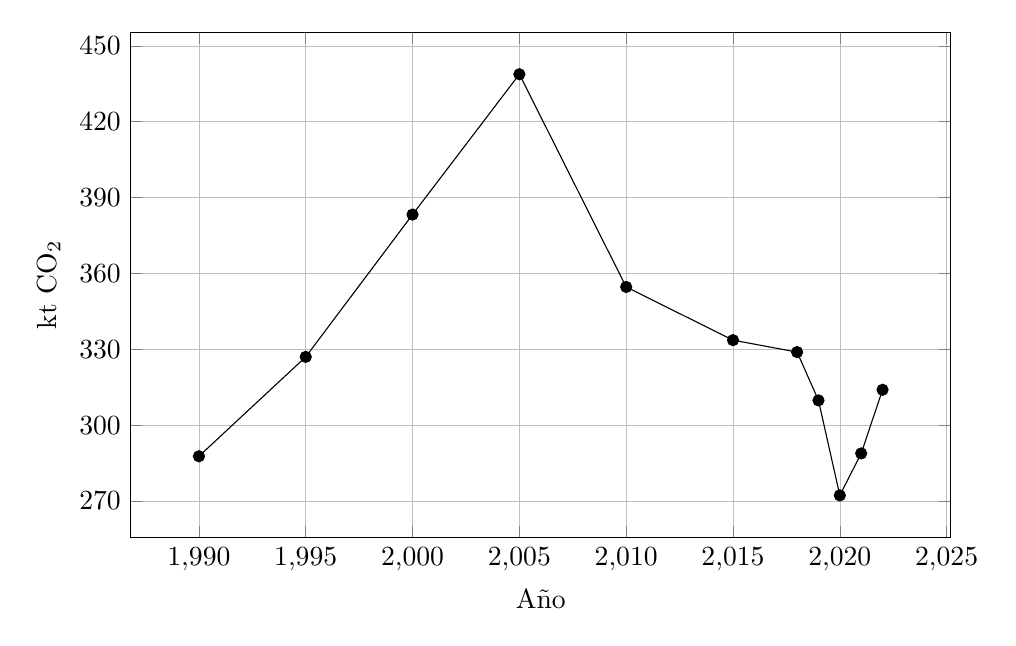
\begin{tikzpicture}
		\begin{axis}[
			xlabel={Año},
			ylabel={kt CO\textsubscript{2}},
			xtick={1990,1995,2000,2005,2010,2015,2020,2025},
			ytick={270, 300, ..., 450},
			grid=both,
			grid style={line width=.1pt, draw=gray!10},
			major grid style={line width=.2pt,draw=gray!50},
			width=12cm,
			height=8cm,
			]
			\addplot[mark=*] coordinates {
				(1990, 287.710)
				(1995, 327.011)
				(2000, 383.276)
				(2005, 438.760)
				(2010, 354.652)
				(2015, 333.623)
				(2018, 328.905)
				(2019, 309.814)
				(2020, 272.244)
				(2021, 288.848)
				(2022, 314.000)
			};
		\end{axis}
	\end{tikzpicture}

\end{figure}

En cuanto a las emisiones asociadas a la generación eléctrica:
\begin{table}[H]
	\centering
	\begin{tabular}{p{3cm}l*{11}{c}}
		\toprule
		tCO\textsubscript{2} $\times$ 1.000.000& 2011 & 2012 & 2013 & 2014 & 2015 & 2016 & 2017 & 2018 & 2019 & 2020 & 2021 & 2022 \\
		\midrule
		Carbón &   41,0 & 51,1 & 37,5 & 41,1 & 50,0 & 35,4 & 42,8 & 36,0 & 12,4 & 4,9 & 4,9 & 7,5 \\
		Fuel + Gas  &  0,0 & 0,0 & 0,0 & 0,0 & 0,0 & 0,0 & 0,0 & 0,0 & 0,0 & 0,0 & 0,0 & 0,0 \\
		Motores diésel &  2,9 & 2,9 & 2,7 & 2,6 & 2,7 & 2,8 & 2,7 & 2,2 & 2,0 & 1,6 & 1,7 & 1,7 \\
		Turbina de gas &  0,9 & 1,0 & 0,7 & 0,8 & 0,7 & 0,5 & 0,7 & 1,0 & 0,7 & 0,4 & 0,5 & 0,7 \\
		Turbina de vapor &  2,3 & 2,4 & 2,2 & 1,8 & 2,0 & 2,3 & 2,4 & 2,2 & 2,0 & 1,3 & 1,0 & 1,1 \\
		Ciclo combinado  & 21,0 & 16,4 & 11,4 & 10,5 & 12,0 & 12,0 & 14,9 & 11,8 & 21,2 & 17,1 & 17,4 & 26,2 \\
		Cogeneración  &  11,6 & 12,3 & 11,7 & 9,2 & 9,6 & 9,8 & 10,7 & 11,0 & 11,3 & 10,1 & 9,7 & 6,6 \\
		Residuos no renovables &  0,3 & 0,4 & 0,4 & 0,5 & 0,6 & 0,6 & 0,6 & 0,6 & 0,5 & 0,7 & 0,8 & 0,6 \\
		Total Emisiones &  80,1 & 86,4 & 66,6 & 66,5 & 77,6 & 63,5 & 74,9 & 64,9 & 50,0 & 36,1 & 35,9 & 44,4 \\ 
		\\
		\hline
		\\
		Factor de emision de CO\textsubscript{2} (tCO\textsubscript{2}/MWh) &  0,29 & 0,31 & 0,24 & 0,25 & 0,29 & 0,24 & 0,29 & 0,25 & 0,19 & 0,15 & 0,14 & 0,16 \\
		\bottomrule
	\end{tabular}
\end{table}

En cuanto a los rendimientos de diversas plantas de generación eléctrica:
\begin{table}[h]
	\label{tab:conversion-efficiency}
	\begin{tabular}{lcccc}
		\toprule
		&Eficiencia conversión&\multicolumn{3}{c}{Emisiones en gramos/kWh} \\
		\cline{3-5}
		&  (\%) & NOx & SO2 & CO2 \\
		\midrule
		Carbón pulverizado (sin descontaminar S) & 36 & 1.29 & 17.2 & 884 \\
		Carbón pulverizado (con descontaminación S) & 36 & 1.29 & 0.86 & 884 \\
		Carbón en lecho fluidificado & 37 & 0.42 & 0.84 & 861 \\
		Ciclo combinado de carbón gasificado & 42 & 0.11 & 0.3 & 758 \\
		Turbina de gas & 39 & 0.23 & 0 & 470 \\
		Ciclo combinado de turbina de gas & 53 & 0.1 & 0 & 345 \\
		\bottomrule
	\end{tabular}
\end{table}

\section{Protocolo de Kioto}
\subsection{Políticas y medidas}
\subsection{Creación de sumideros}
\subsection{Mecanismos flexibles}